\chapter{Zerbitzu-langileak (Service Worker-ak)}
\index{Service Worker}
Service Worker-a (SW) nabigatzailean, atzeko planoan eta web orririk gabe exekutatzen den \mbox{script} bat da. Script hauek egikaritzeko ez da behar ez erabiltzailearen interakziorik ezta web orririk ere. Ezaugarri horri esker, Service Worker-ak Interneteko konexiorik gabe geratzen garenean erabiltzaileari beste zerbait eskaintzeko erabil ditzakegu. Adibidez, demagun erabiltzailea inprimaki batean mezu bat idazten ari denean konexioa galdu egiten duela. Idazten ari zen mezu hori bidali nahiko balu, inprimakian bidali botoian sakatu eta... mezua galdu egingo du! Ez badugu ezer programatzen egoera hori ekiditeko, mezua galdu egingo da erabiltzailea konexiorik gabe baitago. Hemen sartzen da Service Worker APIa. SW batek konexiorik ez dagoela antzeman dezake eta mezua nabigatzailearen katxean gorde, erabiltzaileari ohartaraziz konexiorik gabe dagoela (baina mezua ez duela galdu). Konexioa berriro lortzean Service Worker-ak egoera berria antzeman eta gordeta zituen mezu guztiak zerbitzarira bidal ditzake (sinkronizazioa lortuz). Gai honetan, hain zuzen ere, deskribatutako konexiorik gabeko (\textit{offline}\index{offline}) egoera hori kudeatzen ikasiko dugu.

\section{Service Worker-ak nola erabili}

Gure adibidea prestatuko dugu. Hasteko, webgune bat kargatzean, konexioa baldin badago, \ref{fig:serviceworker1}. irudiko egoera bistaratu nahiko dugu, alegia, ikur bat eta konexioa dagoela dioen mezu bat.
\begin{figure}[ht]
	\centering
\begin{tikzpicture}
\node[anchor=south west,inner sep=0] (image) at (0,0)
   {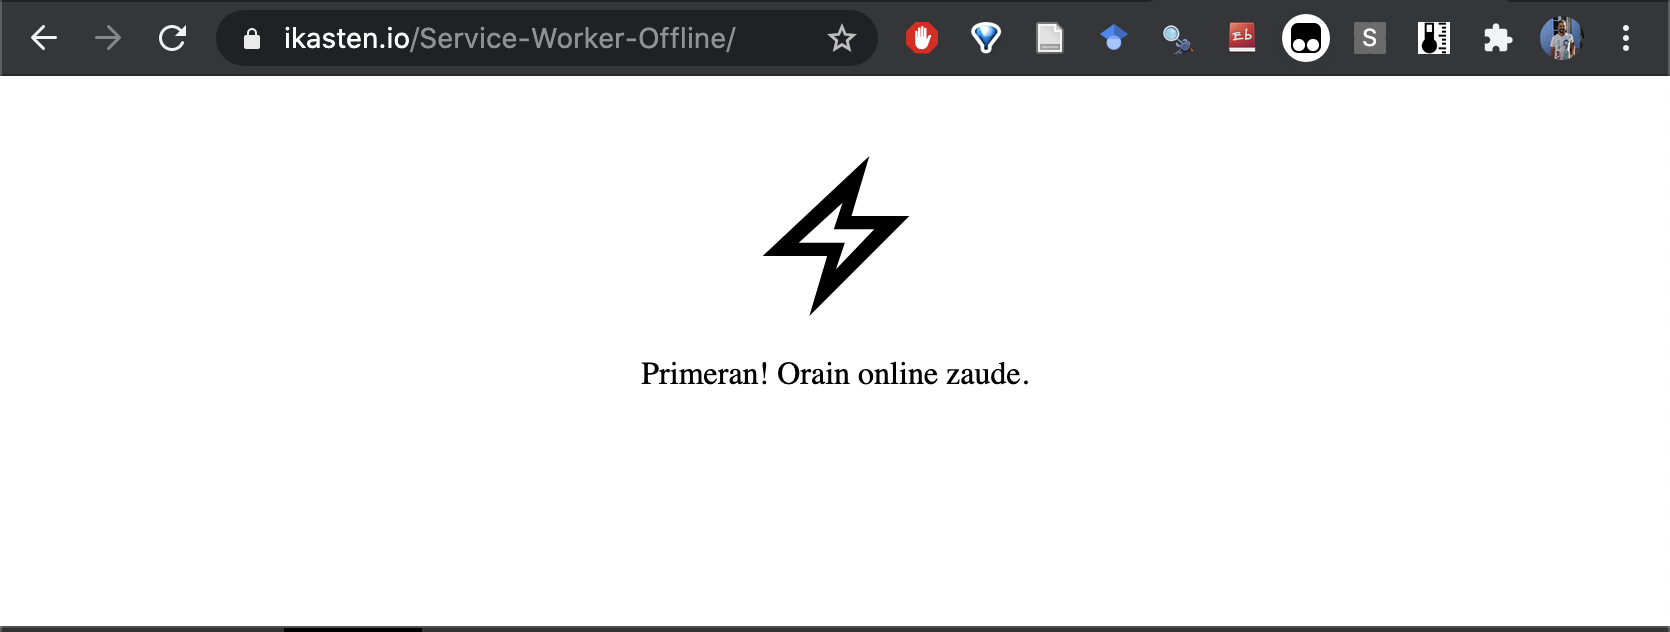
\includegraphics[trim=0cm 0cm 0cm 0cm, clip=true, width=0.75\textwidth]{img/online.png}};
\end{tikzpicture}
\caption{Service Worker-a konexioa dagoenean kargatzen da eta nabigatzailearen atzeko planoan exekutatzen geratzen da (egoiliar).}
\label{fig:serviceworker1}
\end{figure}

Baina konexioa galtzean, erabiltzaileak orri bera kargatzen badu, \ref{fig:serviceworker2}. irudian agertzen den ikurra eta mezua ikustea nahiko dugu.

\begin{figure}[ht]
	\centering
\begin{tikzpicture}
\node[anchor=south west,inner sep=0] (image) at (0,0)
   {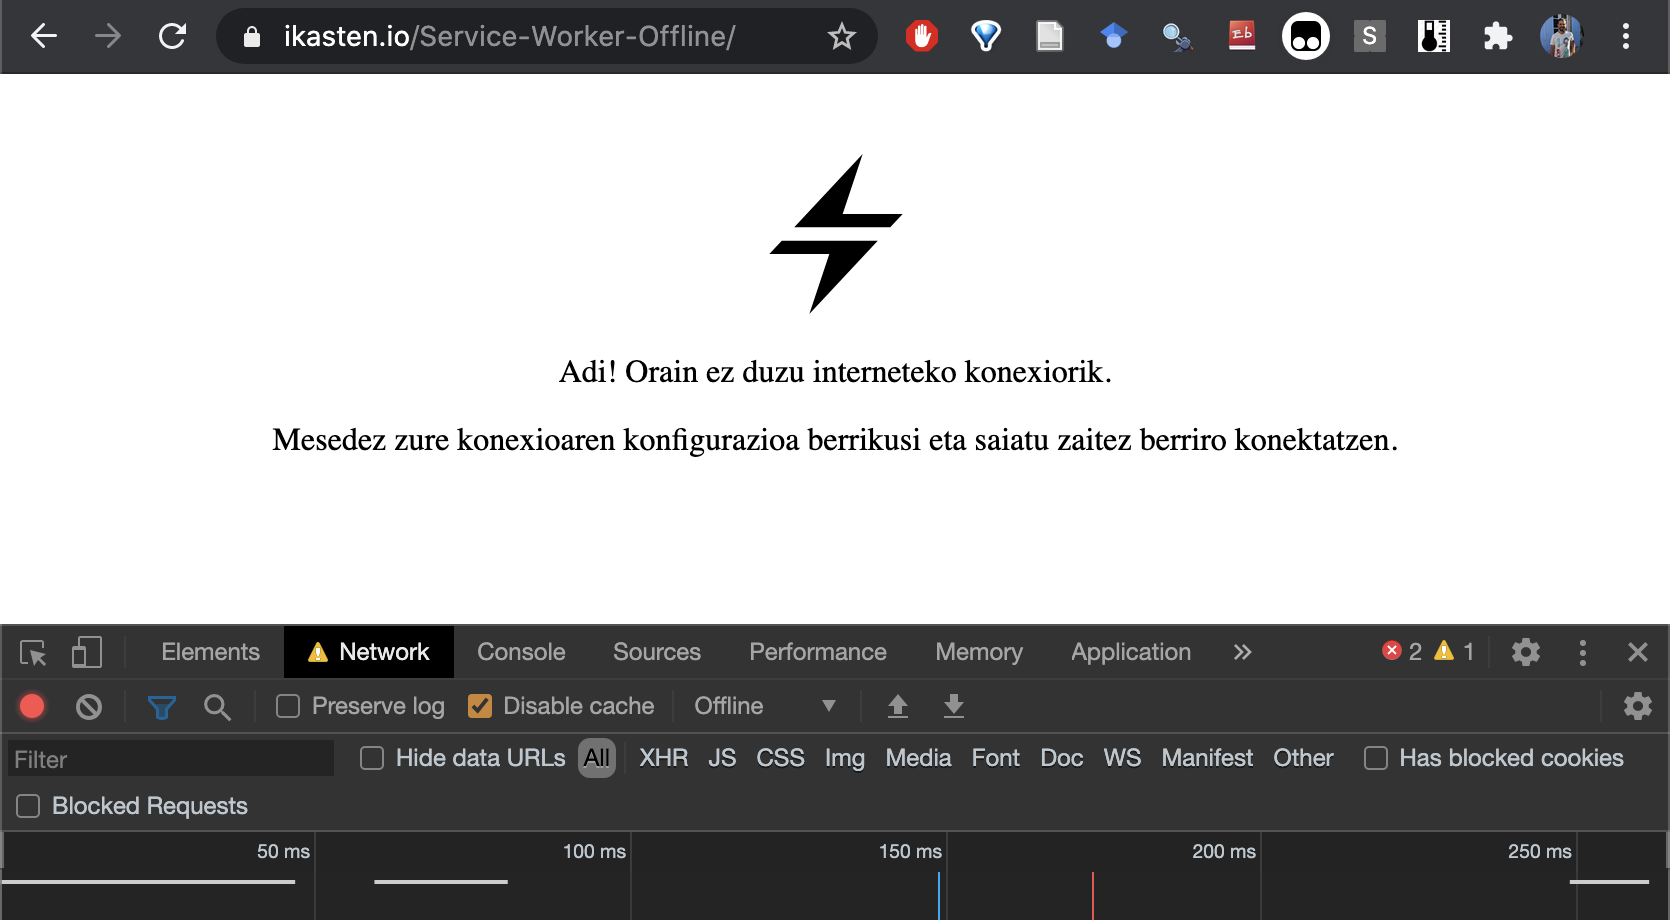
\includegraphics[trim=0cm 0cm 0cm 0cm, clip=true, width=0.75\textwidth]{img/offline.png}};
\end{tikzpicture}
\caption{Service Worker bat probatzeko konexioa eten egin behar dugu. Horretarako Chrome-k Network fitxan \textit{Offline} egoerara jauzi egiteko aukera ematen du.}
\label{fig:serviceworker2}
\end{figure}

Service Worker-a hasierako orria kargatzean nabigatzailearen atzeko planoan geratzen da egoiliar. Hortik, \index{proxy} \textit{proxy} baten lanak egiten ditu (\ref{fig:serviceworker3}. irudia) Hau da, web aplikazioak HTTP(s) eskaera bat egiten duenean SWatik igaroko da eta horrek hortik aurrera konexioak monitorizatuko ditu, proxy baten lanak eginez. Konexioa badago (\textit{online} egoeran bagaude), SWa gardena izango da, dagokion webgunetik baliabidea eskatuko du eta aplikazioari itzuliko dio. Konexioa galtzen bada (\textit{offline} egoera), alternatiba bat \textit{cache} batetik jasoko du eta hori izango da aplikazioan bistaratuko dena. Hurrengo ataletan prozesu hau nola inplementatzen den ikasiko dugu.

\begin{figure}[ht]
	\centering
\begin{tikzpicture}
\node[anchor=south west,inner sep=0] (image) at (0,0)
   {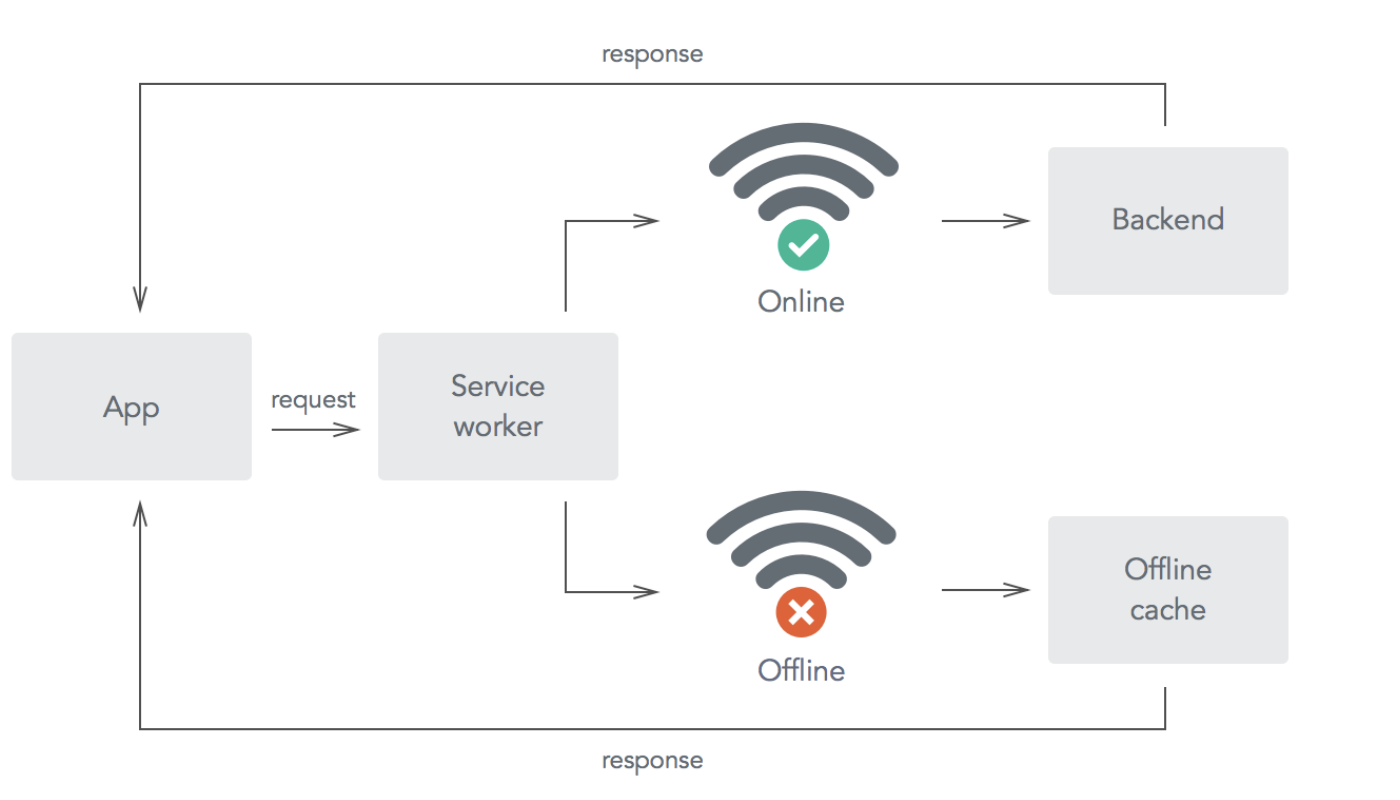
\includegraphics[trim=0cm 0cm 0cm 0cm, clip=true, width=0.75\textwidth]{img/serviceworker3.png}};
\end{tikzpicture}
\caption{Service Worker batek proxy-aren lanak egiten ditu \textit{fetch} eskaerak antzematen. Konexioa dagoenean, urruneko zerbitzariari birbidaliko dizkio eskaerak. Ez dagoenean, \textit{cache} batetik jasoko ditu. Iturria: \href{https://auth0.com/blog/creating-offline-first-web-apps-with-service-workers/}{https://auth0.com/blog/creating-offline-first-web-apps-with-service-workers/}.}
\label{fig:serviceworker3}
\end{figure}

\section{Konexiorik gabeko aplikazioak}

Aipatutako konexiorik gabeko aplikazioa lortzeko, hiru fasetan banatuko ditugu eman beharreko pausoak:

\begin{itemize}
    \item SWa instalatu eta \textit{cache}an \textit{offline} orria txertatu (\textit{offline} egoeran ikusi behar den orriaren kopia bat).
    \item Erabiltzailea konexiorik gabe nabigatzen saiatzen bada, \textit{cache}an dagoen orria itzuli.
    \item Erabiltzaileak konexioa izanik orrian nabigatzen badu, zerbitzaritik jasoko du orriaren edukia (SWrik egongo ez balitz bezala).
\end{itemize}

\section{Service Worker-a instalatu}

Service Worker-a instalatzeko honako scripta erabiliko dugu.

\begin{lstlisting}[language=JavaScript]
<script>
		// Service Worker-a erregistratu
		if ('serviceWorker' in navigator) {
			navigator.serviceWorker.register('./service-worker.js')
			.then(function(registration) {
		        // Ondo erregistratu da
		        console.log('ServiceWorker-a irismen honekin erregistratu da: ', registration.scope);
		}).catch(function(err) {
		    // Erregistroak kale egin du  :(
		    	console.log('ServiceWorker-a ezin izan da erregistratu: ', err);
		    });
		}
	</script>
\end{lstlisting}
\index{scope}
Bertan ServiceWorker-a uneko nabigatzailean onartzen den edo ez egiaztatu ondoren (3. lerroa), erregistratu egiten da, promes baten bidez. Erregistratzeko\index{register} \hl{navigator.serviceWorker.register} metodoa erabiliko dugu. Metodo horrek parametro gisa SWaren kodea duen scriptaren bidea jasoko du. Parametro hori garrantzitsua da. Adibidean, \textquotesingle{}./\textquotesingle{} (uneko katalogoa); alegia, uneko karpetaren barruan egiten diren eskaerak monitorizatuko dituela soilik (haren irismena \textquotesingle{}./\textquotesingle{} dela esango dugu). Edo teknikoki, \textit{fetch}\index{fetch} gertaerak soilik \textquotesingle{}./\textquotesingle{} karpetan monitorizatuko direla. Horren ordez, bidea  \hl{/adibidea/service-worker.js} izango balitz, irismena soilik \hl{/adibidea/} karpetaren barrukoa izango litzateke.

SW bat hainbat aldiz erregistratzen saiatuz gero, ez da ezer gertatuko (nabigatzaileak behin bakarrik erregistratuko du).  

\section{ServiceWorker-a programatzen}

SWa programatzeko garbi izan behar dugu haren funtzionamendua (ikus \ref{fig:serviceworker4}. irudia). ServiceWorker bat irismen baten barruan erregistratu ondoren, irismen horren barruan dagoen eskaera berriak jasotzen hasiko da.


\begin{figure}[ht]
	\centering
\begin{tikzpicture}[framed]
\node[anchor=south west,inner sep=0] (image) at (0,0)
   {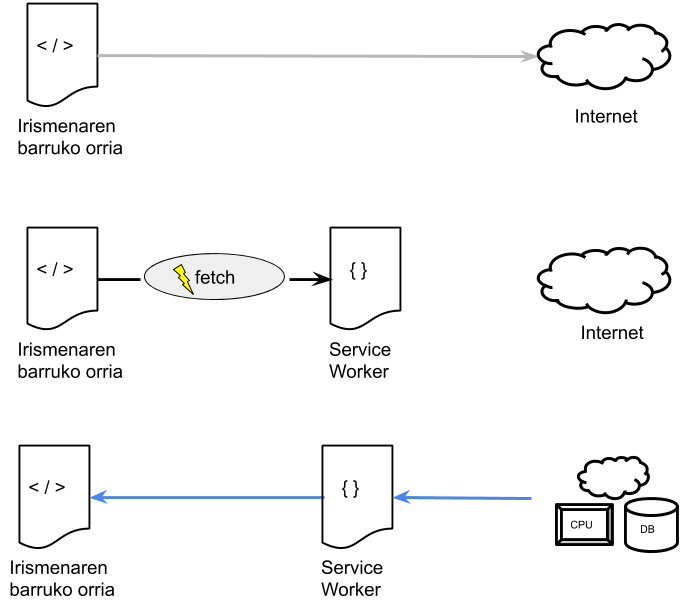
\includegraphics[trim=0cm 0cm 0cm 0cm, clip=true, width=0.75\textwidth]{img/serviceworker4.png}};
\end{tikzpicture}
\caption{\textit{Fetch} gertaerak antzeman eta gero SWak erabaki egin behar du nondik jaso horiei erantzuteko balioak: Internetetik (konexioa badago), cache batetik edo zuzenean sortu programa baten bidez (konexiorik izan ezean).
Iturria:  https://developer.mozilla.org/en-US/docs/Web/API/Service\_Worker\_API/Using\_Service\_Workers.}
\label{fig:serviceworker4}
\end{figure}


 Eskaera horiei erantzuteko SWak \index{respondWith} \hl{event.respondWith()} metodoa erabiliko du, erantzunaren objektua parametro gisa pasatuz. Erantzun-objektu horren edukia betetzeko hiru aukera ditu: 1) konexioa badago, eskaera dagokion zerbitzariari bidaliko dio eta horren erantzuna bueltatuko du. 2) Konexiorik egon ezean, SWak \textit{cachea} erabil dezake erantzuna eraikitzeko, edo 3) zuzenean, erantzuna eraiki script bat exekutatuz.

\section{\textit{Cache}-memoria betetzen}

Azter dezagun SWaren hasierako prozedura \textit{offline} edukia \textit{cache}an gordetzeko. Horretarako, \hl{caches}\index{caches} objektua erabiliko du, alegia, nabigatzaileak iraunkortasuna lortzeko eskaintzen duen mekanismo bat.

\begin{lstlisting}[language=JavaScript]
let cacheVersion = 1;
let currentCache = {
  offline: 'offline-cache' + cacheVersion
};
const offlineUrl = 'offline-page.html';

this.addEventListener('install', event => {
  event.waitUntil(
    caches.open(currentCache.offline).then(function(cache) {
      return cache.addAll([
          './img/offline.svg',
          offlineUrl
      ]);
    })
  )});
\end{lstlisting}

\index{install}\hl{Install} gertaeran (alegia, SWa exekutatzen den lehendabiziko aldian), \textquotesingle{}offline-cache1\textquotesingle{} izeneko \textit{cachea} ireki (izen hori guk erabaki dugu) eta bertan bi baliabide gordeko ditu (\hl{cache.addAll}\index{cache.addAll} metodoari bi elementuren arraya pasatuz): ``/img/offline.svg'' (ikurra) eta offline-page.html (konexiorik gabe gaudenean bistaratu nahi dugun HTML orria). \textit{Cachea}n sartutako fitxategi horiek \ref{fig:serviceworker5}. irudian ikus daitezke. \hl{waitUntil}\index{waitUntil} metodoak (8. lerroa) promes bat hartzen du parametro gisa eta promes hori bete arte itxarongo du. Promesa bi modutara bete daiteke: \textit{cachean} gorde diren fitxategi guztiak ondo instalatzen badira, zuzen beteko da (\textit{resolved})\index{resolved}; cachean ezin izan bada fitxategiren bat sartu, errore batekin beteko da eta SWa ez da instalatuko (\textit{rejected})\index{rejected}.

\begin{figure}[ht]
	\centering
\begin{tikzpicture}[framed]
\node[anchor=south west,inner sep=0] (image) at (0,0)
   {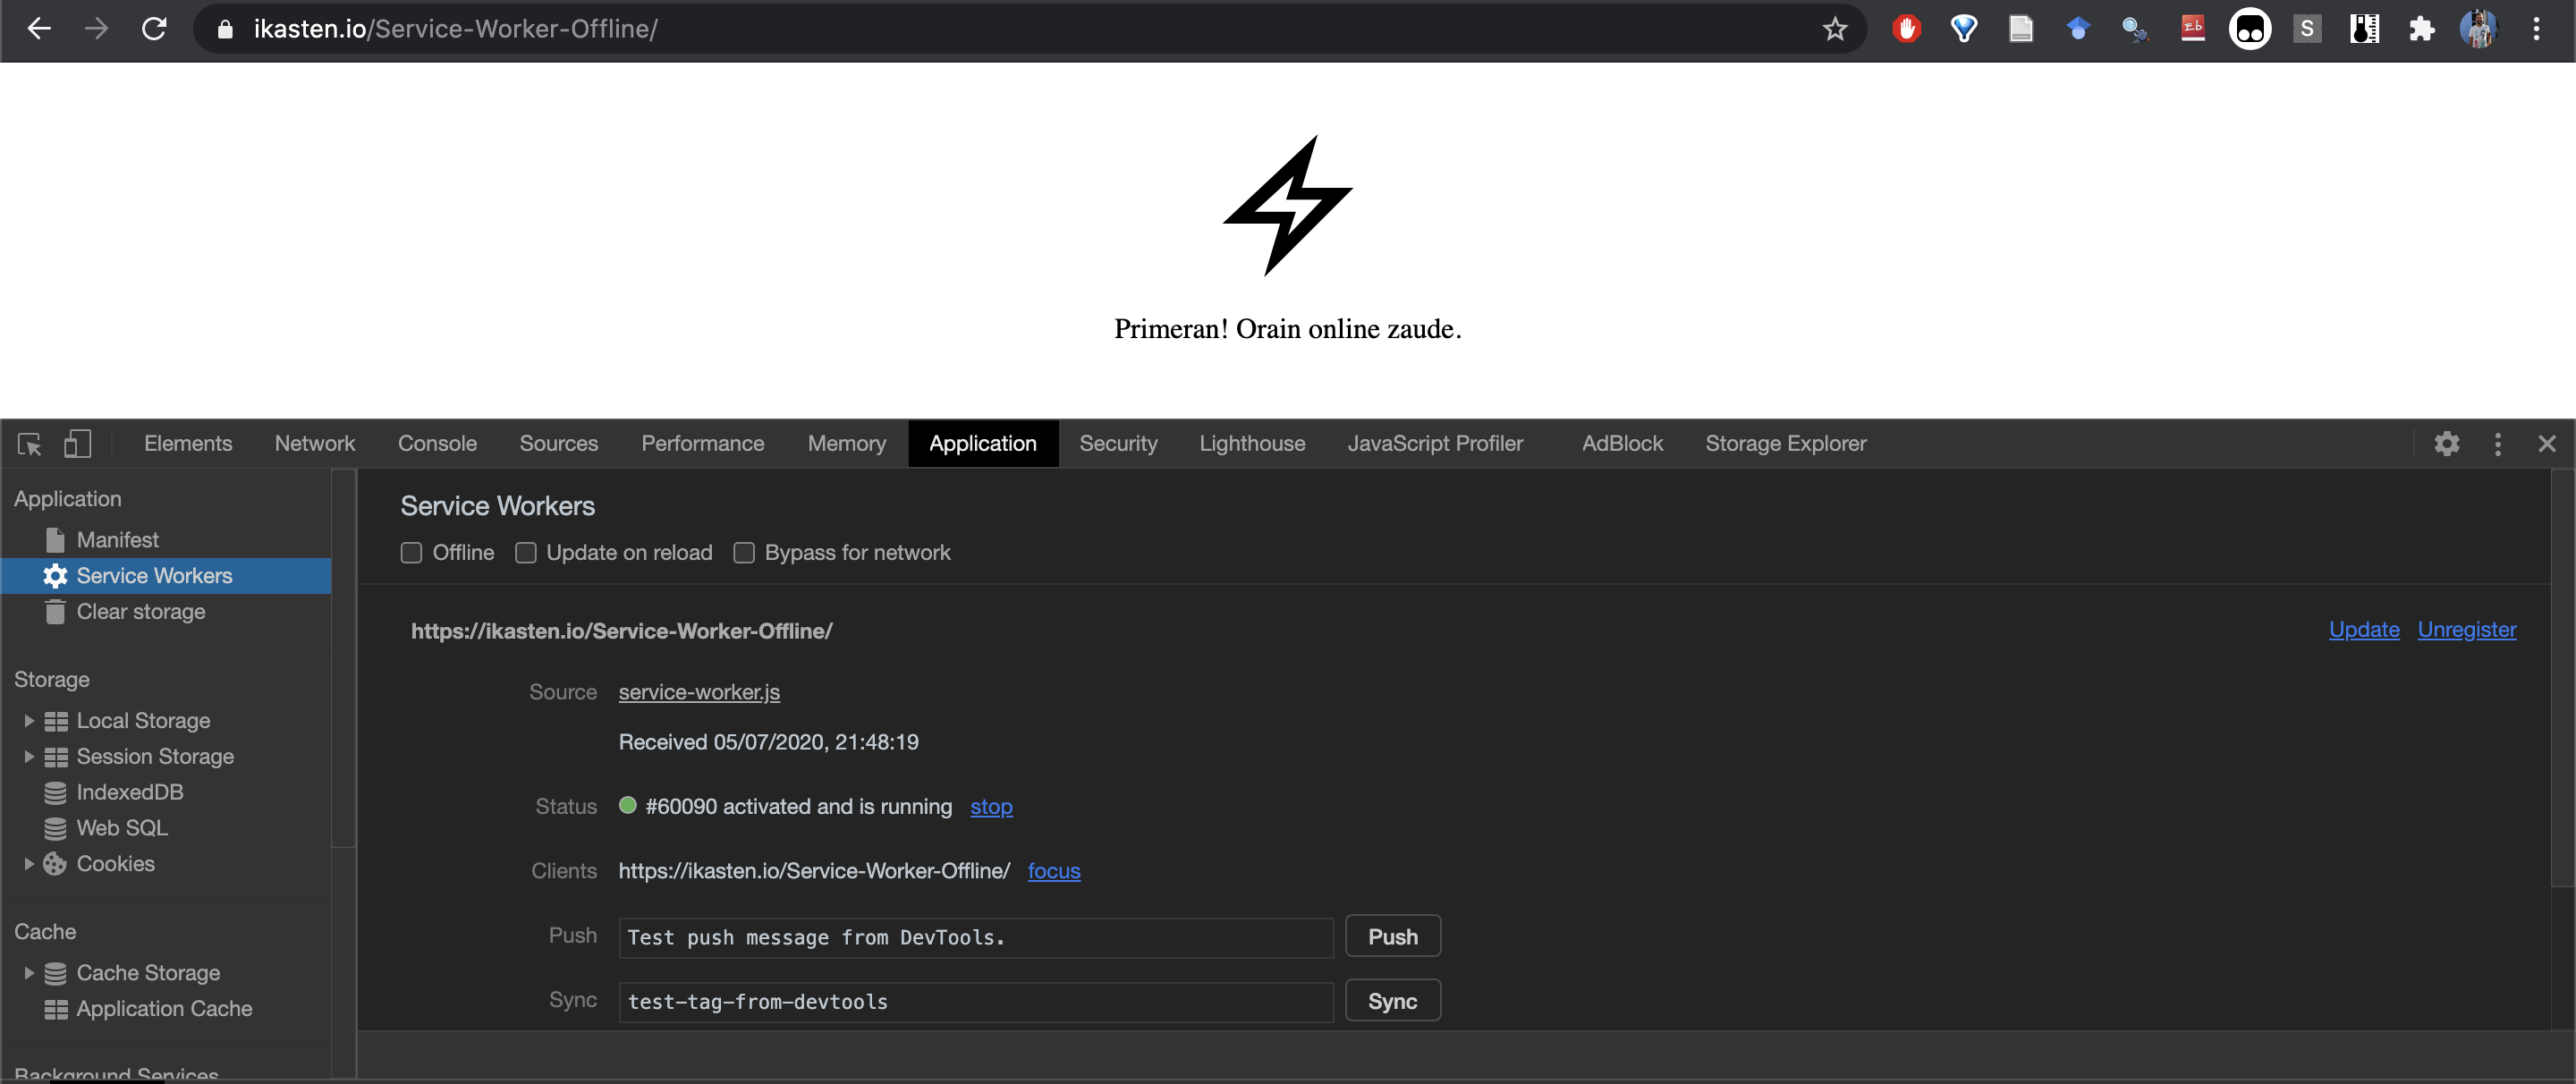
\includegraphics[trim=0cm 0cm 0cm 0cm, clip=true, width=0.75\textwidth]{img/serviceworker5.png}};
\end{tikzpicture}
\caption{Service Worker-ak kudeatzeko edo arazteko DevTools tresnak atal berezia dauka \hl{Application/Service Workers} fitxan.}
\label{fig:serviceworker5}
\end{figure}

\begin{figure}[ht]
	\centering
\begin{tikzpicture}[framed]
\node[anchor=south west,inner sep=0] (image) at (0,0)
   {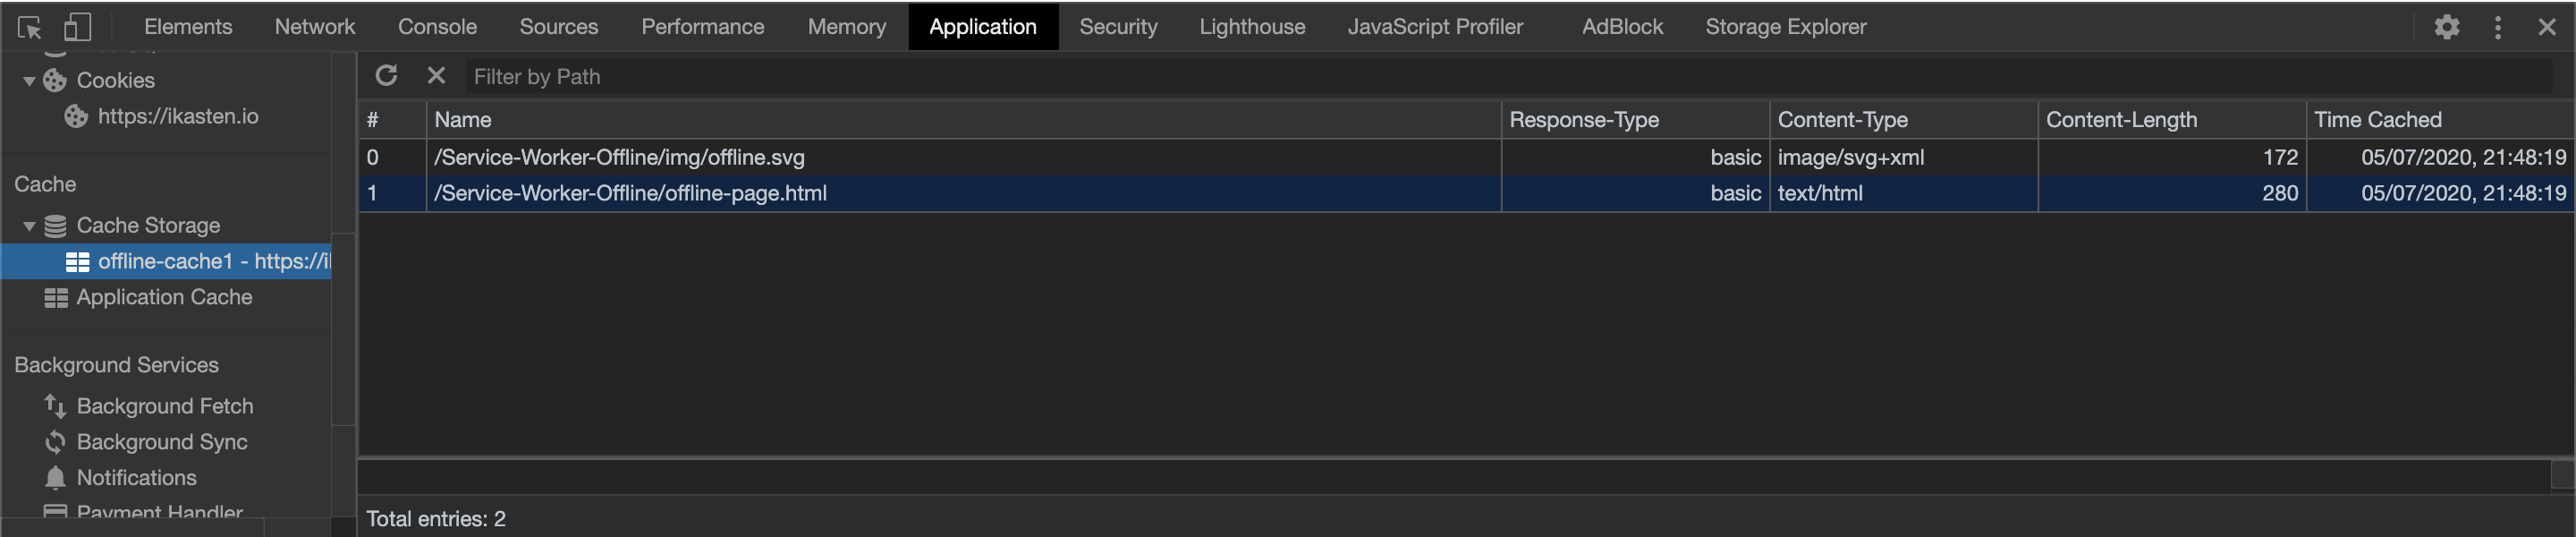
\includegraphics[trim=0cm 0cm 0cm 0cm, clip=true, width=1.0\textwidth]{img/offlinecache.png}};
\end{tikzpicture}
\caption{\textit{Offline Cachea}-ren edukia ikusteko DevTools tresnak atal berezi bat eskaintzen du \hl{Application/Cache/Cache Storage} fitxan.}
\label{fig:serviceworker6}
\end{figure}

Behin instalatuta dagoenean, SWak monitorizatu egingo ditu erabiltzailearen mugimenduak (irismenaren barruan dauden mugimenduak). Alegia, beste orri batera joateko estekan sakatzean \textit{fetch} gertaera altxatuko da eta SWak jasoko du. 

Bertan, SWak HTML orri bat eskatu den begiratuko du eta horrela balitz aipatutako \hl{event.respondWith} metodoaz baliatuko da erantzuna emateko. Hurrengo kode-adibidean,  8. lerroan SWak \hl{fetch()} metodoari deituko dio, urruneko zerbitzaritik eskatutako baliabidea jaitsi nahian. Ezin badu (konexiorik ez dagoelako, adibidez), salbuespen bat altxatuko da, \textit{catch} blokean tratatuko dena. Bertan SWak \textit{cache}tik \textit{offlineUrl}-a jaso eta erabiltzaileari bidaliko dio erantzun gisa.

\index{caches.match}
Ohart gaitezen offlineUrl-ak SVG bat erabiltzen duela (ez HTML orri bat), beraz, irudi hori jaisteko \textit{fetch} gertaera datorrenean SWa \textit{if} baldintzaren \textit{else} adarretik sartuko da (12. lerroa). Hor SVGa \textit{cache}an dagoen begiratuko du eta horrela balitz (kasu honetan bai, badago), cachean dagoen baliabidea itzuliko du erantzun gisa. Ez balego, \textit{fetch()} metodoari deituko lioke Internetetik atzitu nahian (eta hor ere ez balego, errore bat emango luke).

\begin{lstlisting}[language=JavaScript]
this.addEventListener('fetch', event => {
  // request.mode = navigate ez dago eskuragarri nabigatzaile guztietan
  // horregatik sartu dugu baldintza alternatibo bat
  // Accept: text/html goiburua aztertuz
  if (event.request.mode === 'navigate' || (event.request.method === 'GET' && event.request.headers.get('accept'). includes('text/html'))) {
        event.respondWith(
          fetch(event.request.url).catch(error => {
              // offline orria bueltatu
              return caches.match(offlineUrl);
          })
    );
  }
  else{
        // erantzun ahal denarekin (cache-tik edo hor ez balego,
        // internetetik (noski, konexioa badago, bestela errore bat jasoko dugu)
        event.respondWith(caches.match(event.request)
                        .then(function (response) {
                        return response || fetch(event.request);
                    })
            );
      }
});
\end{lstlisting}

Gai honetan zehar landu dugun adibidearen kodea Dean Hume erabiltzailearen GitHubeko biltegi honetan oinarritu da: 
\href{https://github.com/deanhume/Service-Worker-Offline}{https://github.com/deanhume/Service-Worker-Offline}.

Adibidearen inplementazioa hemen proba dezakezu: \href{https://ikasten.io/Service-Worker-Offline/}{https://ikasten.io/Service-Worker-Offline}.


Adibidea probatzeko, Chromen DevTools ireki eta bertan Network fitxan sakatu. Jarraian, aukera-zerrendan \textit{online} egoeratik \textit{offline} egoerara pasa (ikus \ref{fig:serviceworker6}. irudia).
\begin{figure}[ht]
	\centering
\begin{tikzpicture}[framed]
\node[anchor=south west,inner sep=0] (image) at (0,0)
   {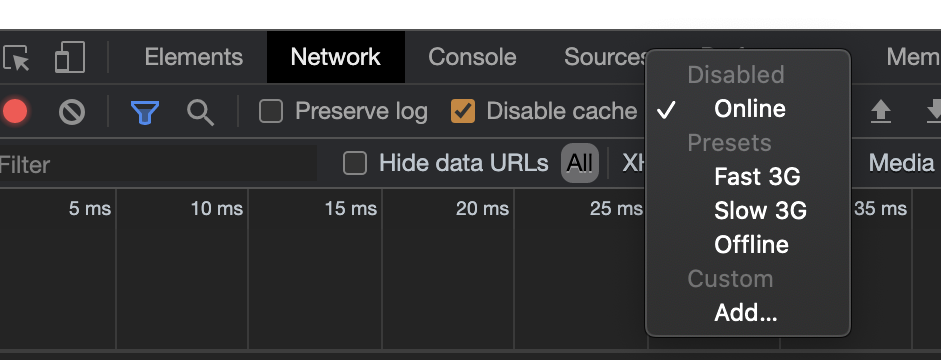
\includegraphics[trim=0cm 0cm 0cm 0cm, clip=true, width=0.75\textwidth]{img/serviceworkers/sw6.png}};
\end{tikzpicture}
\caption{Google Chromek Online egoeratik Offline egoerara jauzia egiteko aukera ematen digu. Service Worker APIarekin probak egiteko ezin egokiagoa.}
\label{fig:serviceworker6}
\end{figure}

\textit{Offline} gaudelarik orria birkargatzen badugu, SWak egoera antzemango du eta \textit{offline} bertsioa erakutsiko digu (ikus \ref{fig:serviceworker7}. irudia).

\begin{figure}[ht]
	\centering
\begin{tikzpicture}[framed]
\node[anchor=south west,inner sep=0] (image) at (0,0)
   {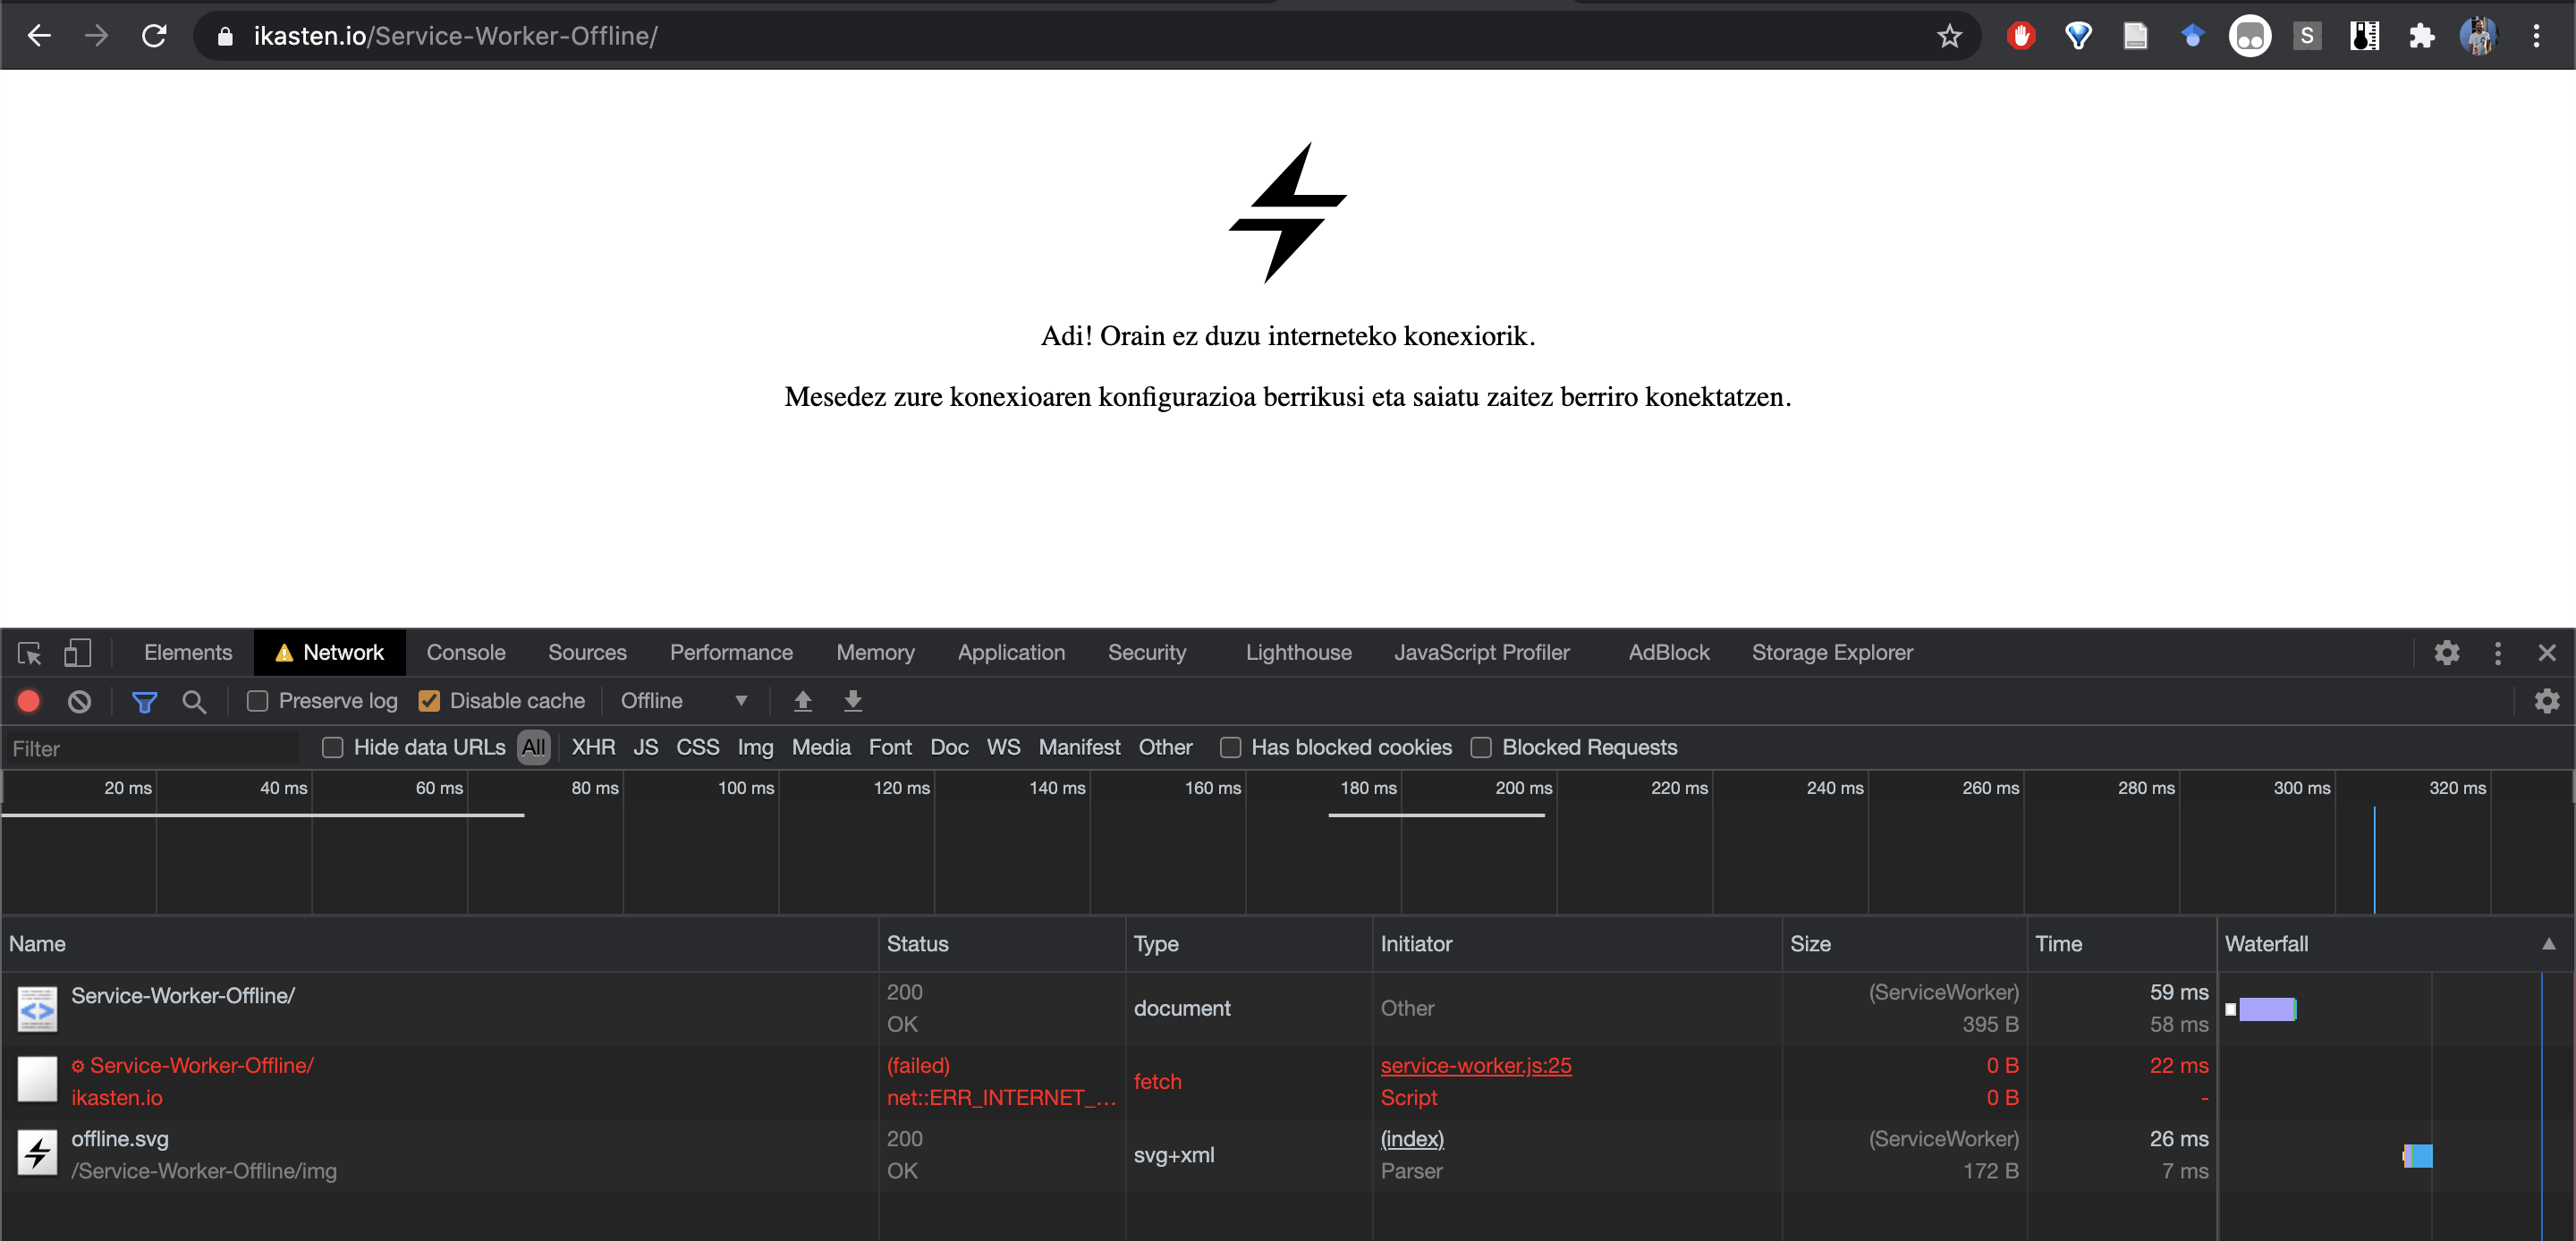
\includegraphics[trim=0cm 0cm 0cm 0cm, clip=true, width=0.75\textwidth]{img/serviceworkers/sw7.png}};
\end{tikzpicture}
\caption{Interneteko konexiorik gabe gaudenean Service Worker batek \textit{offline-cachea}n dugun edukia bistara dezake, eta horrekin erabiltzaileak lan egiten jarrai dezake, konexioa bueltatu arte.}
\label{fig:serviceworker7}
\end{figure}

\section{Ariketa}
Gai honetan azaldu den adibidea inplementatu eta probatu, bai Chrome-n nola Firefox-en. 

Ohart zaitez Firefox-en, Chrome-n bezala, lineaz kanpo lan egiteko aukera bat ere badugula Web Garapenerako menuaren azken lerroan (ikus \ref{fig:lineazkanpo}. irudia).


\begin{figure}[ht]
	\centering
\begin{tikzpicture}[framed]
\node[anchor=south west,inner sep=0] (image) at (0,0)
   {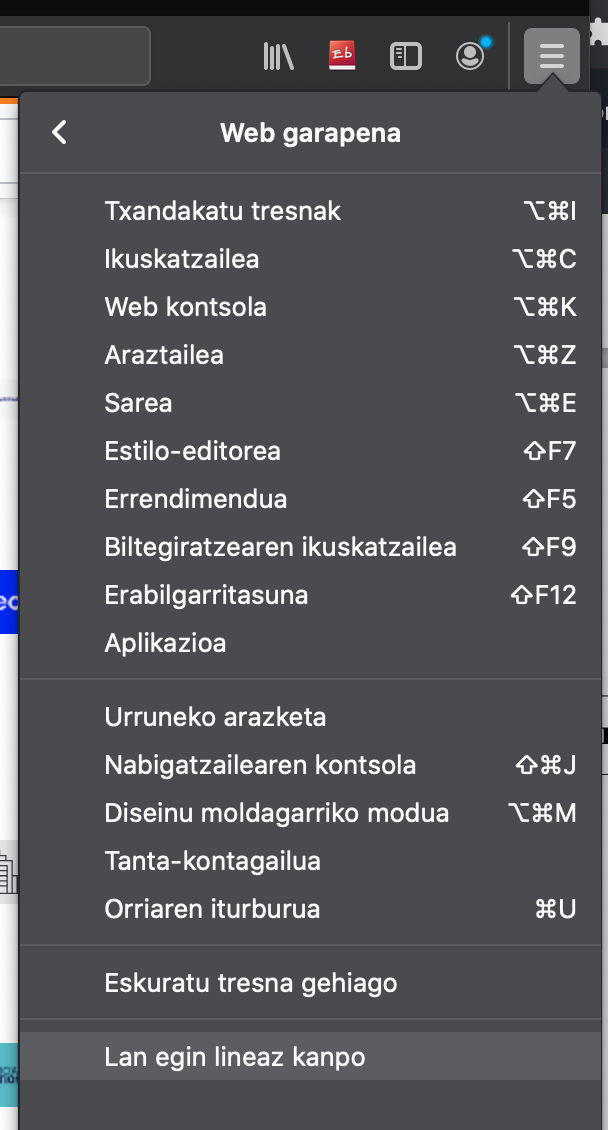
\includegraphics[trim=0cm 0cm 0cm 0cm, clip=true, width=0.5\textwidth]{img/serviceworkers/lineazkanpo.png}};
\end{tikzpicture}
\caption{Firefox-en eta Chrome-n \textit{throttling} izeneko aukerak ditugu, alegia, konexio-abiaduraren baldintzak simulatzeko aukerak. Firefox-en, berriz, konexiorik gabe lan egiteko aukera menu honetan isolatuta dago.}
\label{fig:lineazkanpo}
\end{figure}
